%%%%%%%%%%%%%%%%%%%%%%%%%%%%%%%%%%%%%%%%%%%%%%%%%%%%%%%%%%%%%%%%%%%%%%%%
%    INSTITUTE OF PHYSICS PUBLISHING                                   %
%                                                                      %
%   `Preparing an article for publication in an Institute of Physics   %
%    Publishing journal using LaTeX'                                   %
%                                                                      %
%    LaTeX source code `ioplau2e.tex' used to generate `author         %
%    guidelines', the documentation explaining and demonstrating use   %
%    of the Institute of Physics Publishing LaTeX preprint files       %
%    `iopart.cls, iopart12.clo and iopart10.clo'.                      %
%                                                                      %
%    `ioplau2e.tex' itself uses LaTeX with `iopart.cls'                %
%                                                                      %
%%%%%%%%%%%%%%%%%%%%%%%%%%%%%%%%%%
%
%
% First we have a character check
%
% ! exclamation mark    " double quote  
% # hash                ` opening quote (grave)
% & ampersand           ' closing quote (acute)
% $ dollar              % percent       
% ( open parenthesis    ) close paren.  
% - hyphen              = equals sign
% | vertical bar        ~ tilde         
% @ at sign             _ underscore
% { open curly brace    } close curly   
% [ open square         ] close square bracket
% + plus sign           ; semi-colon    
% * asterisk            : colon
% < open angle bracket  > close angle   
% , comma               . full stop
% ? question mark       / forward slash 
% \ backslash           ^ circumflex
%
% ABCDEFGHIJKLMNOPQRSTUVWXYZ 
% abcdefghijklmnopqrstuvwxyz 
% 1234567890
%
%%%%%%%%%%%%%%%%%%%%%%%%%%%%%%%%%%%%%%%%%%%%%%%%%%%%%%%%%%%%%%%%%%%
%

%AIP Reprint Class%%%%%%%%%%%%%%%%%%%%%%%%%%%%%%%%%%%%%%%%%%%%%%%%%%%%%%%%%%%%%%%%%%%%%%%%%%%%%
\documentclass[aip,prl,amsmath,amssymb,reprint,superscriptaddress]{revtex4-1} %preprint version
\usepackage{graphicx}% Include figure files
\usepackage{dcolumn}% Align table columns on decimal point
\usepackage{bm}% bold math
\usepackage{epstopdf}

    \renewcommand{\topfraction}{0.9}    % max fraction of floats at top
    \renewcommand{\bottomfraction}{0.8}    % max fraction of floats at bottom
    \setcounter{topnumber}{2}
    \setcounter{bottomnumber}{2}
    \setcounter{totalnumber}{4}     % 2 may work better
    \setcounter{dbltopnumber}{2}    % for 2-column pages
    \renewcommand{\dbltopfraction}{0.9}    % fit big float above 2-col. text
    \renewcommand{\textfraction}{0.07}    % allow minimal text w. figs
    \renewcommand{\floatpagefraction}{0.7}    % require fuller float pages
    \renewcommand{\dblfloatpagefraction}{0.7}    % require fuller float pages
    \setlength{\abovecaptionskip}{5pt}
    \setlength{\belowcaptionskip}{5pt}
    \setlength{\parskip}{0pt}
    \setlength{\textfloatsep}{5pt} 

%%%%%%%%%%%%%%%%%%%%%%%%%%%%%%%%%%%%%%%%%%%%%%%%%%%%%%%%%%%%%%%%%%%%%%%%%%%%%%%%%%%%%%%%%%%%%%%%%%

%IOP preprint class %%%%%%%%%%%%%%%%%%%%%%%%%%%%%%%%%%%%%%%%%%%%%%%%%%%%%%%%%%%%%%%%%%%%%%%%%%%%%%
%\documentclass[12pt]{iopart}
%\newcommand{\gguide}{{\it Preparing graphics for IOP journals}}
%Uncomment next line if AMS fonts required
%\usepackage{iopams}
%\usepackage{graphicx}
%\usepackage{epstopdf}  
%%%%%%%%%%%%%%%%%%%%%%%%%%%%%%%%%%%%%%%%%%%%%%%%%%%%%%%%%%%%%%%%%%%%%%%%%%%%%%%%%%%%%%%%%%%%%%%%%%
%Slava's inserts %%%%%%%%%%%%%%%%%%%%%%%%%%%%%%%%%%%%%%%%%%%%%%%%%%%%%%%%%%%%%%%%%%%%%%%%%%%%%%
%\usepackage{amsfonts}
%\usepackage{amssymb}

%\newcommand{\ptt}[1]{\frac{\partial#1}{\partial t}}
%\newcommand{\vvec}{\mathbf{v}}
%\newcommand{\Bvec}{\mathbf{B}}
%\newcommand{\Evec}{\mathbf{E}}
%\newcommand{\Jvec}{\mathbf{J}}
%\newcommand{\Avec}{\mathbf{A}}
%%%%%%%%%%%%%%%%%%%%%%%%%%%%%%%%%%%%%%%%%%%%%%%%%%%%%%%%%%%%%%%%%%%%%%%%%%%%%%%%%%%%%%%%%%%%%%%%%%

\begin{document}
\title{Variance Anisotropy in a laboratory plasma}

\author{D.A. Schaffner}
\affiliation{Swarthmore College, Swarthmore, PA, USA}
\author{M.R. Brown}
\affiliation{Swarthmore College, Swarthmore, PA, USA}
\author{V.S. Lukin}
\affiliation{Space Science Division, Naval Research Laboratory, Washington, DC, USA}

\date{\today}
\begin{abstract}
Variance anisotropy observed in magnetic fluctuations on the Swarthmore Spheromak Experiment (SSX).
\end{abstract}

\maketitle

\section{Introduction}

The solar wind turbulence community has seen a flurry of results in recent years, as diagnostic capabilities on spacecraft have steadily improved, especially in the temporal resolution which has allowed for investigation into ion, sub-ion and electron scale turbulence measurements. In addition, newer analysis techniques have been developed to better tap the details of the rich turbulent environment that is the heliosphere. 

Theoretical treatments of magnetized plasma turbulence have almost universally predicted anisotropy to develop based on directions perpendicular and parallel to a mean field vector; many forms of this anisotropy has been predicted and observed (a good overview of the various types is given in Horbury 2012)~\cite{horbury12}. This paper focuses on variance anisotropy---the observation of greater magnetic fluctuation power in components perpendicular to the mean magnetic field versus parallel. From the experimentalist point of view, this is the most straightforward quantity to report and a reasonable place to begin. Analysis of other forms of anisotropy are saved for future work.---%has garnered great interest as it is viewed as a keystone result for theoretical understanding of MHD turbulence. 

Anisotropy is a common theme in solar wind turbulence and is predicted to be present by many turbulence theories. Since the solar wind speeds are typically super-Alfvenic, anisotropy studies generally reference the velocity vector of the bulk flow when defining perpendicular versus parallel fluctuations. Variance anisotropy, however, references a mean magnetic field vector---either global or local mean.

As results from space become more detailed, comparison to simulation and laboratory experiment become more useful in order to better develop the theory as well as inform future space missions. Experiments conducted in the MHD wind-tunnel configuration of the Swarthmore Spheromak Experiment have shown the ability to produce and analyze MHD turbulence using many of the same methods used in the space plasma community, and has produced turbulence measurements which are comparable to \textit{in-situ} results~\cite{schaffner14a}. Moreover, using varying amounts of helicity injection, some characteristics of the turbulence can be modified~\cite{schaffner14b}.

A full spectral analysis of fluctuations in the SSX has been conducted, including magnetic field, density and Mach flow fluctuations. Using a wavelet transform method to decompose the timeseries signal, the magnetic field fluctuation spectra can be broken into portions that are parallel or perpendicular to the local magnetic field vector. Analysis of these portions show that parallel fluctuation power decreases slightly faster than that for perpendicular fluctuations generating a separating in power as a function of increasing frequency. This effect in frequency space is very close to the observation of variance anisotropy seen in wavenumber space in solar wind turbulence. The ratio is shown to grow from nearly isotropic levels in the energy injection scale to a maximum $\perp/\parallel$ ratio of 3 at frequencies of about 1MHz. Beyond this point, the ratio begins to contract reaching isotropy around 10MHz. Though the axial flow speeds of the plasma in the wind-tunnel sub-Mach, if a Taylor hypthesis were still invoked this peak in the ratio would correspond to the ion inertial scale length. Comparison between magnetic flucutation spectra and flow fluctuation spectra are also reported.

The organization of this paper is as follows: First, a brief description of the plasma laboratory is given. Then, an overview of the analysis techniques used to determine perpendicular and parallel fluctuations is provided; details of the method and a second method used to verify its validity are described in the appendix. The results of this analysis is provided in section 4 including how spectra scaling varies with helicity injection, and how it evolves in time. In section 5 a comparison of magnetic fluctuation spectra is made to velocity and density fluctuations as well. Section 6 gives a discussion of how all of these spectra results are consistent with the observation of an ion inertial scale in the plasma. Comparison to a MHD simulation is made in section 7 and conclusions are presented in section 8.

\section{Experiment}

The results center around three groupings of experimental parameters of 40 shots each enumerated by a stuffing flux value. The main run has a stuffing flux value of 1.0mWb. It has average field values of 5kG and average bulk flow of M=0.6. A second run has a value of 0.5mWb, and had average field values of 5kG, but a Mach number of only 0.2. A third run has zero stuffing flux, low field values, and flows of M=0.2.

\section{Analysis Techniques}

\section{Variance Anisotropy}

The magnetic field fluctuation spectra perpendicular and parallel to the local magnetic field vector is shown in figure~\cite{fig:spectra}(a) averaged over 40 shots and the inner four probe tips. Like previously reported magnetic spectra~\cite{schaffner14}, both perpendicular and parallel curves exhibit power-law like behavior for most frequencies between 10kHz and 10MHz. Fits can be made to various sections of the curve using a Maximum Likelihood Estimation method~\cite{clauset09}; the short fits show that the scaling appears to gradually change from spectral indices of about 1 in the injection (or outer) range and from about 2.5 to 5 in the remaining sections. As has been noted before, with the exception of the injection range slope, the inertial and possibly dissipation range spectral indices are steeper than observed in solar wind turbulence spectra.

\begin{figure}[!htbp]
\centerline{
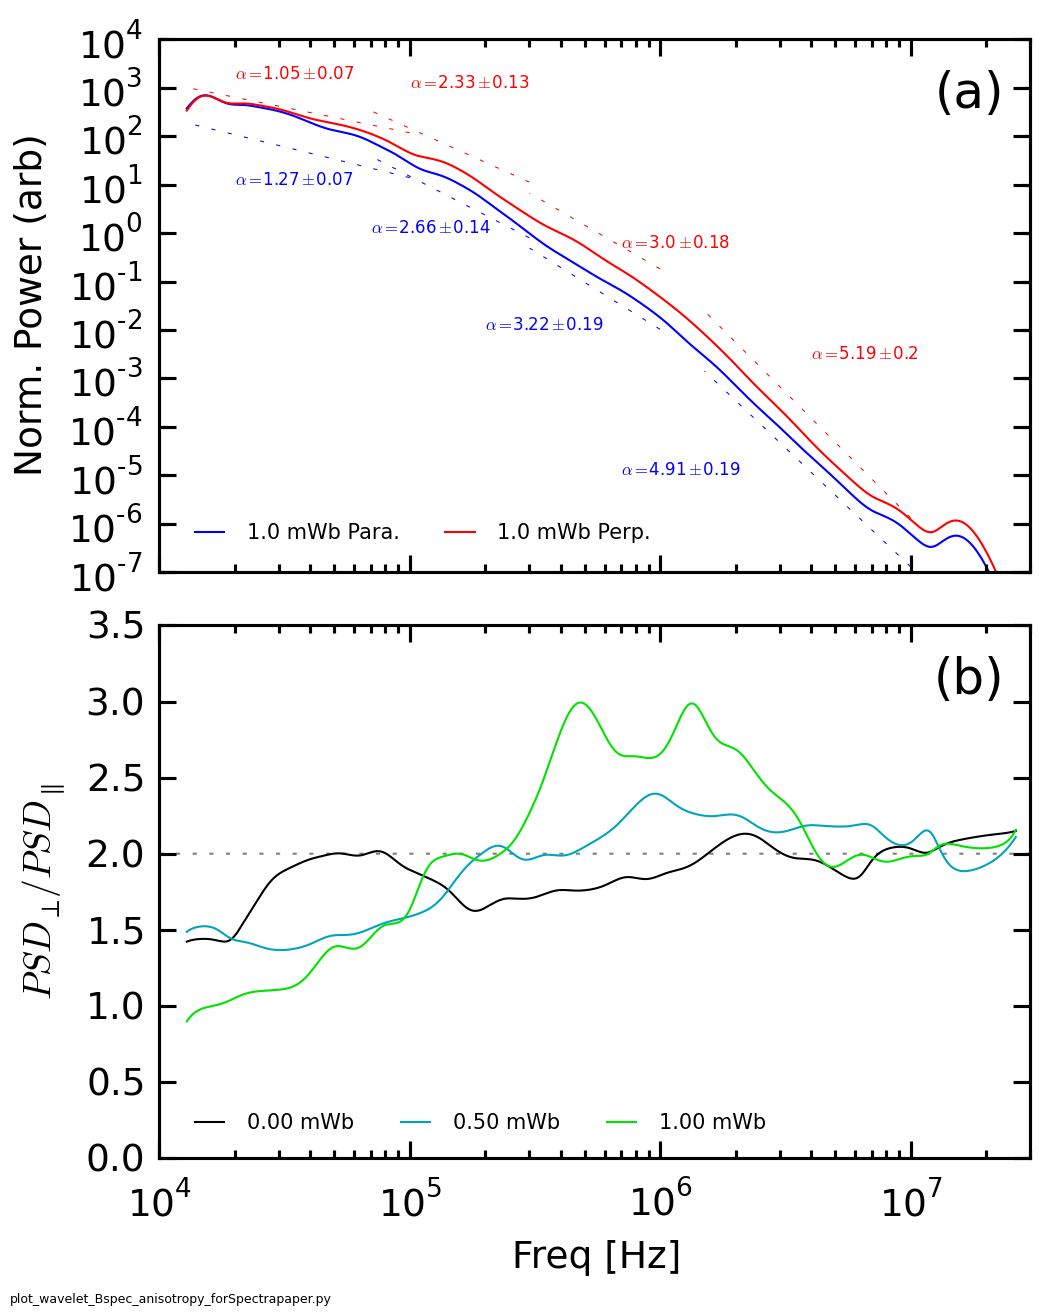
\includegraphics[width=8.5cm]{Bperppara_chan1t4_1mWbspectra_40t60us_wAsymRatio}}
\caption{\label{fig:spectra}}
\end{figure}

However, the separation between perpendicular and parallel spectra proceed in a manner similar to that found in space. Both perpendicular fluctuations (red) and parallel fluctuations (blue) begin at roughly the same magnitude in power. Beyond 20kHz, though, the parallel curve dips down slightly faster than the perpendicular and this trend continues up to about 500kHz. Then the separation begins to decrease and approaches a constant value from 5MHz to the Nyquist limit of 32MHz. This gradual change as a function of frequency is more clearly observed in figure ~\ref{fig:spectra}(b) plotted in log-linear format, which provides the ratio of the two curves in figure~\ref{fig:specta}(a). Since the fluctuations perpendicular to the B-field have two component directions while parallel fluctuations have only one, the point of isotropy, or equal fluctuations in all three components) occurs when the ratio of perpendicular to parallel equal to 2. Isotropy is indicated in figure~\ref{fig:spectra}(b) by the dashed gray line.

At the lowest frequencies, the balance of power actually tips toward parallel over perpendicular. As the frequency decreases, an thus, presumably, the scale size decreases, the ratio approaches isotropy, then changes over to a dominantly perpendicular power level. The ratio continues to steadily increase reaching a peak of about 3 at about 500kHz. There is a brief dip before the ratio rises again at about 1.5MHz; at this point, the ratio begins to drop steadily, and approaches an isotropic level at about 5MHz. 

The scale dependency of the 1.0mWb data can be compared to other helicity levels. The black curve shows the anisotropy ratio for the zero helicity state, when the field strength is about an order of magnitude less, and there is much less structure to the field. As might be expected for such a state, there appear to be very little anisotropy at any scale with values staying close to R=2. The blue curve, showing the anisotropy ratio for a 0.5mWb stuffing case, clearly shows intermediate ratios between the 1.0 and 0.0mWb plasmas. This observation is somewhat curious as there is very little difference in magnetic field magnitude between 1.0mWb and 0.5mWb; the only difference between to the two states is the amount of average flow (which would not be expected to affect anisotropy) and the amount of helicity in the plasma.

\begin{figure}[!htbp]
\centerline{
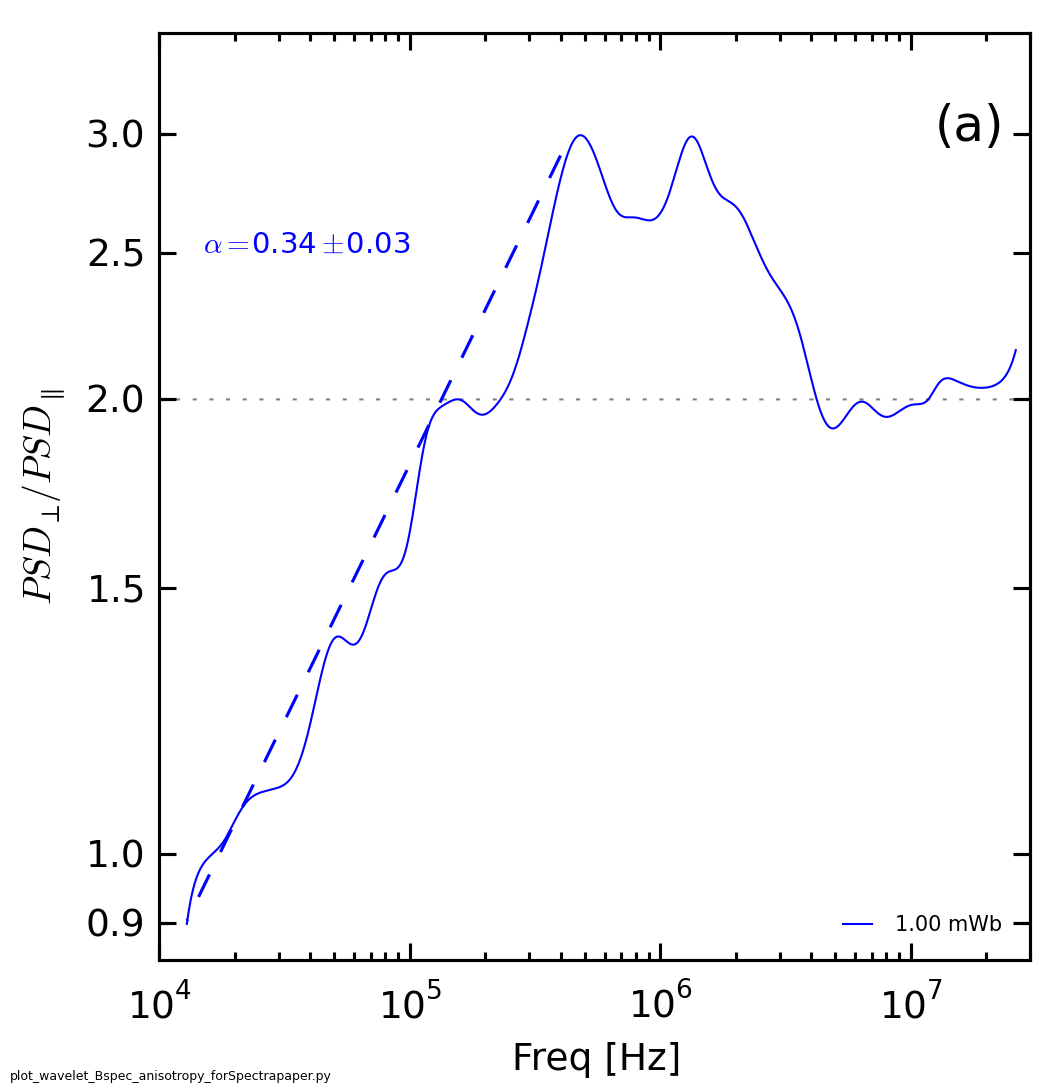
\includegraphics[width=8.5cm]{Bperppara_chan1t4_1mWbspectra_40t60us_AsymRatio_wFit}}
\caption{\label{fig:fitratio}}
\end{figure}

\begin{figure}[!htbp]
\centerline{
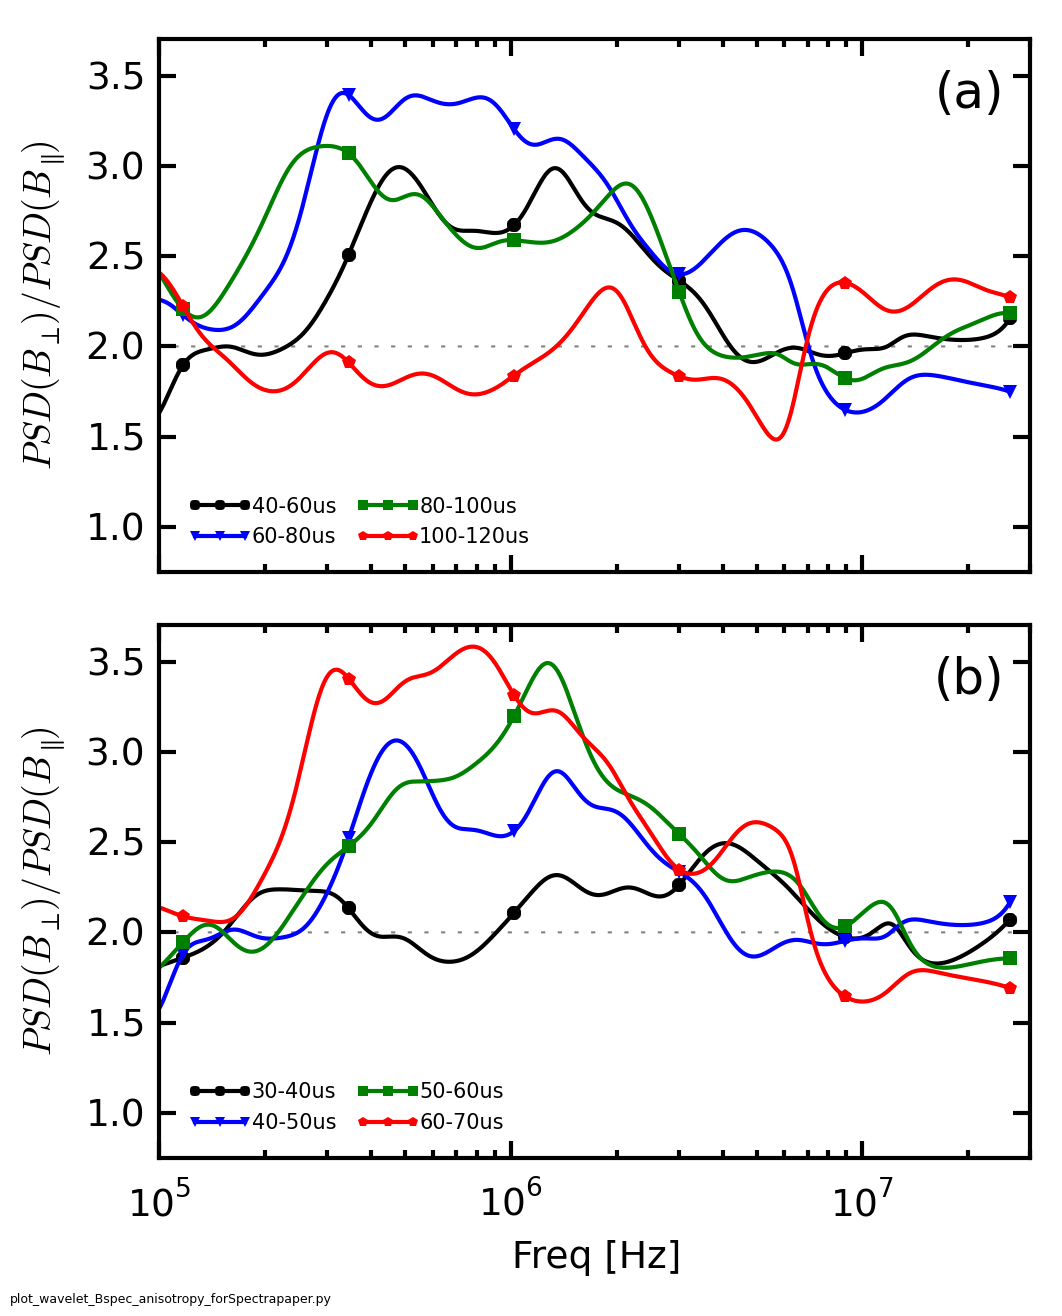
\includegraphics[width=8.5cm]{Bperppara_chan1t4_1mWbspectra_timescan}}
\caption{\label{fig:timeratio}}
\end{figure}

Fits to both the spectra and the ratio are shown in figure~\ref{fig:spectra}. In figure~\ref{fig:spectra}(a), fits are made to four sections of each curve. The spectral indices, error and range of fit for both parallel and perpendicular spectra are shown in the table below. Overall, the spectral indicies are anisotropy; for each section fit, the parallel slope is consistently steeper than the perpendicular slope. This difference is also reflected in the fit shown in figure~\ref{fig:fitratio}. An index of $\alpha = 0.35$ indicates that the ratio scales like $f^{1/3}$ for the region between 10kHz and 500kHz.

An evolution of the anisotropy over time is also observed. Figure~\ref{fig:timeratio}(a) and (b) shows the change of the anisotropy ratio as a function of time ranges of 10$\mu s$ intervals(a) and 20$\mu s$ intervals(b). The black curve in figure~\ref{fig:timeratio} shows a period of time, 30-40$\mu s$, just as the plasma is reaching the midplane probe. The curve remains near isotropic levels for most of the frequencies. As time increases in 10$\mu s$ intervals, the perpendicular power clearly increases in the 100kHz to 1MHz range, while decreases in the 10-100kHz range. The actually peaks highest in the time frame just beyond the main analysis period shown in figure~\ref{fig:spectra}(b). These trends demonstrate that the anisotropy increases as more time is allowed for the turbulence to evolve. Figure~\ref{fig:timeratio}(b), shows that after energy is no longer being injected to maintain the turbulence, the anisotropy decreases. After 100$\mu s$, the magnetic field fluctuations have return to isotropy.

\section{Flow and Density Spectra}

\section{Discussion and Evidence for Ion Scale Effects}

\section{Comparison with Simulation}

\section{Conclusions}

\appendix

\section{Computation of Variance Anisotropy}

% ----------------------------------------------------------------
\section*{Acknowledgements}
%  We gratefully acknowledge many useful discussions with William Matthaeus. This work has been funded by the US DoE Experimental Plasma Research program and the National Science Foundation.  The simulations were performed using the advanced computing resources (Cray XC30 Edison system) at the National Energy Research Scientific Computing Center.
% ----------------------------------------------------------------
\section*{References}
\begin{thebibliography}{99}

\bibitem{horbury12} T.S. Horbury, R.T. Wicks, C.H.K. Chen Anisotropy in Space Plasma Turbulence: Solar Wind Observations. Space Sci Rev. {\bf 172} 325-342 (2012).

\bibitem{schaffner14a} D.A. Schaffner {\it et al.} Turbulence analysis of an experimental flux rope plasma. Accepted by Plas. Phys. Cont. Fusion. Dec 2013.

\bibitem{schaffner14b} D.A. Schaffner {\it et al.} Observation of turbulent intermittency scaling with magnetic helicity in an MHD plasma wind-tunnel. Submitted to PRL? Feb 2014.

\bibitem{clauset09}A. Clauset, C. Rohilla Shalizi, M.E.J. Newman, Power-law distributions in empirical data, SIAM Rev. {\bf 51}, 661703 (2009).

%\bibitem{Belmabrouk98} Belmabrouk, H., and M. Michard (1998), Taylor length scale measurement by laser Doppler velocimetry, Exp. Fluids, 25, 69Ð76.

%\bibitem{Matthaeus05} Matthaeus, W. H. and Dasso, S. and Weygand, J. M. and Milano, L. J. and Smith, C. W. and Kivelson, M. G., Phys. Rev. Lett. 95, 231101 (2005) Spatial Correlation of Solar-Wind Turbulence from Two-Point Measurements

%\bibitem{Weygand07} Weygand, J. M., Matthaeus, W. H., Dasso, S., Kivelson, M. G., and Walker, R. J. (2007), J. Geophys. Res., 112, A10201.

%\bibitem{Weygand09} Weygand, J. M., Matthaeus, W. H., Dasso, S., Kivelson, M. G., Kristler, L. M., and Mouikis, C. (2009), J. Geophys. Res., 114, A07213.

%\bibitem{Weygand10} Weygand, J. M., Matthaeus, W. H., El-Alaoui, M., Dasso, S., and Kivelson, M. G. (2010), J. Geophys. Res., textit115, A12250.

%\bibitem{Weygand11} Weygand, J. M., Matthaeus, W. H., Dasso, S., and Kivelson, M.G. (2011), J. Geophys. Res., 116, A08120.

%\bibitem{Matthaeus08} Matthaeus W. H., Weygand, J. M., Chuychai, P., Dasso, S., Smith, C. W., and Kivelson, M. (2008), Astrophys. J., 678, L141.

%\bibitem{frisch95}Frisch, U. 1995, {\it Turbulence} (Cambridge: Cambridge Univ. Press)

%\bibitem{sorrisovalvo99}Sorriso-Valvo, L. {\it et al.} Geophys. Res. Lett. {\bf 26}, 1801–1804 (1999).

%\bibitem{wan12}Wan, M. {\it et al.} ApJ. {\bf 744} 177 (2012).

%\bibitem{sorrisovalvo01}Sorriso-Valvo, L. {\it et al.} Planet. Space Sci. {\bf 49}, 1193–1200 (2001).

%\bibitem{marrelli05}Marrelli, L. {\it et al.} Phys. Plasmas. {\bf 12}, 030701 (2005).

%\bibitem{Greco08}A. Greco, P. Chuychai, W. H. Matthaeus, S. Servidio and P. Dmitruk, Intermittent MHD structures and classical discontinuities, Geophys. Res. Lett. {\bf 35}, L19111 (2008).

%\bibitem{Greco09}Greco, A., Matthaeus, W. H., Servidio, S., Chuychai, P., and Dmitruk, P.: Statistical Analysis of Discontinuities in Solar Wind ACE Data and Comparison with Intermittent MHD Turbulence, ApJ {\bf 691}, L111 (2009).

%\bibitem{Wan09}Wan, M., Oughton, S., Servidio, S., and Matthaeus, W. H.: Generation of non-Gaussian statistics and coherent structures in ideal magnetohydrodynamics, Phys. Plasmas {\bf 16}, 080703 (2009).

%\bibitem{Servidio11b}Servidio, S. {\it et al}, J. Geophys. Res. {\bf 116}, A09102 (2011).

%\bibitem{Gray13} T. Gray, M. R. Brown, and D. Dandurand. Phys. Rev. Lett. {\bf 110}, 085002 (2013). 



%\bibitem{Taylor86} J. B. Taylor, Rev. Mod. Phys. {\bf 58}, 741 (1986).

%\bibitem{Matthaeus80} W.H. Matthaeus and D. Montgomery, Ann. N.Y. Acad. Sci. {\bf 357}, 203 (1980).

%\bibitem{torrence98}C. Torrence, G.P. Compo, A practical guide to wavelet analysis. Bull. Am. Meteorol. Soc. {\bf 79}, 6178 (1998).



%\bibitem{wan12}M. Wan, K. T. Osman, W. H. Matthaeus, and S. Oughton, Investigation of intermittency in magnetohydrodynamics and solar wind turbulence: scale-dependent kurtosis, ApJ {\bf 744}, 171 (2012).

%\bibitem{Gray10}T. Gray, V. S. Lukin, M. R. Brown, C. D. Cothran, Three-dimensional reconnection and relaxation of merging spheromak plasmas, Phys. Plasmas {\bf 17}, 102106 (2010).

%\bibitem{goldstein94}Goldstein, M.L., Roberts, D.A. and Fitch, C.A. Jour. Geo. Res. {\bf 99} 11519-11538 (1994).

%\bibitem{ji95}Ji, H., Prager, S.C. and Sarff, J.S. Phys. Rev. Lett. {\bf 74} 2945 (1995).

%\bibitem{telloni12}Telloini, D. {\it et al.}. ApJ. {\bf 751} 19 (2012).

%\bibitem{matthaeusVelli11}Matthaeus, W.H. and Velli, M. Space Sci. Rev. {\bf 160} 145-168 (2011).

%\bibitem{greco12}A. Greco {\it et al.} ApJ. {\bf 749} 105 (2012).

\end{thebibliography}

\end{document}

